\documentclass{article}
\usepackage[utf8]{inputenc}

\title{Messaging im verteilten Echtzeit-Computing\\[0.2em]Performancevergleich zwischen ZeroMQ und nanomsg}
\author{Youri Seichter, HTW Berlin \\ Prof. Dr. Hermann Heßling, HTW Berlin }

\date{29. April 2021}

\usepackage{natbib}
\usepackage{graphicx}

\renewcommand*\contentsname{Inhaltsverzeichnis}
\renewcommand\refname{Literaturverzeichnis}
\renewcommand{\listfigurename}{Abbildungsverzeichnis}

\begin{document}

\maketitle

\clearpage
\tableofcontents
\clearpage

\section{Einleitung}

Da die vertikale Skalierung von Re\-chen\-re\-ssourc\-en aufwändiger wird, wird
das nutzen von verteilten Re\-chen\-re\-ssourc\-en zunehmend wichtiger. Anstatt
ein Re\-chen\-pro\-blem einer einzelnen re\-chen\-star\-ken Maschine zu geben, kann
die Rech\-en\-kraft vieler Maschinen (Nodes) genutzt werden. Dafür ist es
wichtig die Aufgabe effizient in Teilaufgaben zu unterteilen sowie die
Teilaufgaben und die Nodes auszugeben und einzusammeln. Die
Kommunikation zu den Nodes wird oft über Messaging Protokolle gelößt.

Im Rahmen des Forschungsprojekts ``Grischa'', an der HTW Berlin, wird an
Verteilten Systemen geforscht. Grischa ist ein Schachprogramm, welches
versucht möglichst viele Züge im Vorraus zu evaluieren und dabei, im
Gegensatz zu vielen anderen, ohne Heuristiken oder oder Neuronale Netze
arbeitet. Dafür wird eine Menge an Nodes mittels Grid-Computing genutzt,
die nach den bestmöglichen Zügen suchen. Für die Kommunikation zwischen
den verteilten Rechenressourcen wird derzeit die Messaging Bibliothek
ZeroMQ benutzt.

Ziel dieser Arbeit ist die Analyse von Grischas Messaging-System sowie
die Evaluation von ZeroMQ mittels Gegenüberstellung zu einer alternative
namens ``nanomsg" in den Punkten Geschwindigkeit und Bedienbarkeit.

\section{Analyse}

Grischa wurde historisch mit verschiedenen Kom\-mu\-ni\-ka\-tions\-stra\-te\-gien
be\-trie\-ben, z.B. auch mit Redis \cite{noauthor_redis_nodate}. Die für diese Arbeit relevante
Implementierung, ZeroMQ, besteht aus 3 Teil\-an\-wen\-dun\-gen:

\begin{enumerate}
\def\labelenumi{\arabic{enumi}.}
\itemsep1pt\parskip0pt\parsep0pt
\item  ``GClient'': Zuständig für die Zuteilung der Aufgaben sowie
  Schnittstelle zur Spielfläche/GUI (z.B. XBoard). \cite[p.8]{rosenfeld_messaging_2019}
\item  ``GNode'': Stellt die Worker-Node dar. Nimmt Aufgaben vom GClient
  entgegen und bewertet Spielzüge. Je mehr GNode Instanzen erstellt
  werden, desto mehr Spielzüge können berechnet werden. \cite[p.9]{rosenfeld_messaging_2019}
\item  ``GBroker'': Stellt den Message Broker dar, der die Kommunikation
  zwischen den Anwendungen GClient und GNode handhabt. Zwar kann ZeroMQ
  auch ohne Message Broker arbeiten, er erleichtert jedoch Anmeldung und
  Ausfall von Nodes. Gleichzeitig können GNodes über den GBroker ihre
  Ergebnisse zurück geben. \cite[p. 13]{rosenfeld_messaging_2019}
\end{enumerate}

Für diese Arbeit ist die Message-Basierte Kommunikation von vorrangiger
Bedeutung. Dafür wird ZMQ an zwei Stellen eingesetzt.


\begin{enumerate}
\def\labelenumi{\arabic{enumi}.}
\itemsep1pt\parskip0pt\parsep0pt
\item In der Kommunikation zwischen GNodes und GClients. Dies wird umgesetzt
in Sternförmiger Topologie mit dem XPubXSub Modell. Der Vorteil von PubSub sind die
Topic-gesteuerten Nachrichten via URI Adressierung. Mit einem Broker zwischen Publishern und Subscribern löst man das "Dynamic Discovery Problem". Neue Nodes, egal ob Publisher oder Subscriber, verbinden sich mit diesem Vermittelnden Proxy. Aus PubSub wird so XPubXSub. 
In Grischa wird weitergehend für jede Datenflussrichtung eine Verbindung erstellt, sodass man eine bidirektionale Verbindung besteht. So
So kann jedes Modul mit jedem anderen Modul kommunizieren. \cite[p. 43]{rosenfeld_messaging_2019} Für diese Datenverbindung wird das TCP Protokoll genutzt, da die Anwendungen über das Netzwerk miteinander Kommunizieren müssen.  
\item In der Kommunikation zwischen den internen Modulen der GNode Anwendung. Da hier zwischen den Modulen kommuniziert wird, wird das IPC Protokoll eingesetzt.
\end{enumerate}

\begin{figure}[htbp]
\centering
\includegraphics[width=12cm]{./images/5_10_Topologie_der_Kommunikationspfade_der_verteilten_Anwendung_mit_Modulen.png}
\caption{Topologie der Kommunikationspfade der verteilten Anwendung mit Modulen}
\end{figure}

\section{Planung}
Relevant für die Grischa Anwendung ist weniger die Echtzeit-Verarbeitung
und mehr die Skalierbarkeit auf viele GNodes mit einem weiterhin
Stabilen Nachrichtendurchsatz. Da in Grischa sowohl das TCP als auch das
IPC Protokoll genutzt wird, sollen beide Protokolle untersucht werden.
Desweiteren soll betrachtet werden wie sich der Durchsatz im Verhältnis
zur Nachrichtengröße verhält. Diese Parameter sollen sowohl auf dem
bisherigen System ZeroMQ als auch auf der Alternative nanomsg umgesetzt
werden.

Zusammengefasst sind die untersuchten Parameter:
\begin{itemize}
\itemsep4pt\parskip0pt\parsep0pt
    \item
    Message-Bibliothek (ZeroMQ und nanomsg)
    \item
    Nachrichtengröße (als \texttt{msg\_size} bezeichnet) 
    \item
    Anzahl der Nodes (als \texttt{worker\_count} bezeichnet) 
    \item
  Protokoll (TCP und IPC)
\end{itemize}

Um dem Anwendungsfall von Grischa nachzustellen, wird neben Master-
(Client) und Worker-Nodes auch mit einem Router gearbeitet. Da das
PubSub-Modell die Komplexität durch das Topic-basierte Abbonieren von
Nachrichten erhöht, wird auf Request-Reply zurückgegriffen (ReqRep bzw.,
aufgrund des Brokers, XReqXRep) \cite{noauthor_xsub-xpub_nodate}. Die Architektur ist auf Abbildung \ref{figgure:architecture_testsystem} abgebildet.

\begin{figure}[htbp]
\centering

\includegraphics[width=12cm]{./images/architecture.png}
\caption{Die Architektur des Testsystems}
\label{figgure:architecture_testsystem}
\end{figure}

Desweiteren soll sichergestellt sein, dass die einzigen Unterschiede
zwischen den Implementierungen von ZeroMQ und nanomsg lediglich die
Bibliotheksrelevanten Schnitstellen sind. Die Business-Logik sollte möglichst
gleich sein, um diesseitige Auswirkung auf die Performance
auszuschließen. Die Anwendungen sollen außerdem separat kompiliert
werden damit kein nicht gebrauchter Code das Programm verlangsamt. Außerdem
sollten Unterschiede durch Präprozessordirektiven
ausgeschlossen werden indem die gleiche Programmiersprache mit den
gleichen Compileroptionen verwendet werden.

\section{Durchführung}

Als Programmiersprache für die Implementierungen wurden vorrangig die
nativen implementierungen von ZeroMQ und nanomsg in Betracht gezogen,
damit einem Performanceverlust durch Übersetzungsschichten vorgebeugt
wird. ZeroMQ ist nativ in C++ (libzmq), nanomsg in C geschrieben. Da die
Entwicklung an ZeroMQ bereits 2007 angefangen hat sowie heute deutlich
populärer ist und Version 1.0 von nanomsg erst Mitte 2016 erschienen
ist, gibt es mehrere Wrapper von ZeroMQ in C \cite{noauthor_omq_2007}.
Da man daher davon ausgehen kann dass ZeroMQ
ausgereifter ist, wurde sich auf C als gemeinsame Programmiersprache
festgelegt. Bei nanomsg kann so die native Bibliothek benutzt werden
während bei ZeroMQ czmq als High-Level Language-Binding genutzt wird.

\subsection{Worker}

Zuerst generiert der Worker eine zufällige Zeichenkette zum übertragen
mit der Länge von $2^i$, wobei $i$ bis zum vom Benutzer angegebenen
$max\_msg\_size\_power$ läuft. In die gleiche Nachricht werden die
Metainformationen aus Tabelle \ref{table:msg_header} beigefügt
ohne die Größe zu verändern.

Danach wird die Nachricht mit ZeroMQ bzw. nanomsg abgesendet. Dafür wird
in beiden Fällen eine Art Kontext/Socket erstellt und sich mit dem
Broker verbunden. Die Nachricht wird abgesendet, die Antwort empfangen
und direkt gelöscht. Dieser Senden/Empfangen Ablauf wird
$repetitions$-mal wiederholt (Standardmäßig 8912 mal). Danach werden die
Messagingbibliotheksspezifischen Daten gelöscht.

\subsection{Router}

Der Router beschränkt sich, sowohl bei ZeroMQ als auch bei nanomsg, auf
sehr wenig Code. Daher wurden hier eigene Programme für beide
Bibliotheken implementiert.

Die Schnittstellen von ZeroMQ und nanomsg sind sehr ähnlich. Beide
erschaffen jeweils einen Socket für die Master Node(s) und die Client
Nodes. Diese Sockets werden an eine URI gebunden und schlussendlich wird
ein Proxy (ZeroMQ) bzw. ein ``Device'' (nanomsg) gestartet. Von dortan
werden alle Nachrichten entsprechend weitergeleitet.

\subsection{Client (Master)}

Der Client übernimmt die das Benchmarking selbst. Zuerst initialisiert
er die Verbindung zum Broker. Dann stoppt er die Zeit zum Empfangen,
Verarbeiten und Antworten von $repetitions * clients$ Nachrichten: Wiederholungen sowie Anzahl der Clients (jeweils aus dem Header der
Nachricht entnommen). 

\begin{table}[h!]
\centering
\begin{tabular}{l | l} 
    Inhalt & Beschreibung \\
    \hline
     \texttt{tag} & Flags für die steuerung des Workers \\
     \texttt{client\_id} & Numerische ID des Senders \\
     \texttt{msg\_size} & Message Größe \\
     \texttt{repetitions} & Wiederholungen dieser 
     \texttt{msg\_size}. I.d.R. 8192 \\
     \texttt{worker\_count} & Anzahl gestarteter Clients \\
 \hline
\end{tabular}
\caption{Metainformationen einer Nachricht (Header)}
\label{table:msg_header}
\end{table}

\subsection{Setup}

\subsubsection{Software}

Es werden Datengrößen (\texttt{msg\_size}) zwischen 4 Byte und 64 KiB
untersucht sowie Client Mengen zwischen 1 und 128 - jeweils in quadratischer Reihe. Für
die Auswertung wird eine Teilmenge an Datenreihen ausgewählt sofern es die Darstellung
der Ergebnisse nicht verfälscht. Alle Rohdaten sind im Repository zu finden.

Jeder Datenpunkt (Bibliothek, Protokoll, \texttt{msg\_size}, \texttt{client\_count}) 
wird 10 mal abgebildet. Daraus wird ein Durchschnitt gebildet.

Beide Programme werden mit den Compileroptionen \texttt{-O3} und
\texttt{-march=native} compelliert, um auch Optimierungen wie loops
unrolling sowie AVX2 zu er\-mö\-glich\-en.

Am Benchmarking System wurden keine Änderungen an TCP send/recv buffern, an der Maximum Transmission Unit, am Socket backlog oder der Tramsit queue length vorgenommen. Die Werte sind in Tabelle \ref{table:tcp_settings} dokumentiert.

\begin{table}[h!]
\centering
\begin{tabular}{l | l} 
    Einstellung & Wert \\
    \hline
    TCP recv buffer & 4096	131072 6291456 \\
    TCP send buffer & 4096	16384 4194304 \\
    Socket backlog & 4096 \\
    Maximum Transmission Unit & 65536 \\
    Transmit queue length & 1000 \\
 \hline
\end{tabular}
\caption{Netzwerk Buffer und Parameter}
\label{table:tcp_settings}
\end{table}

\subsubsection{Hardware}
Um den Anwendungsfall von Grid-Computing Nahe zu kommen, wird Server-Grade
Hardware eines Cloud Dienstleisters angemietet. Dabei wurde darauf geachtet dedizierte
Rechenkerne anzumieten, um zu verhindern dass Lastspizen anderer Programme 
auf dem gleichen Physischen Kern die Ergebnisse verfälschen. 

\begin{table}[h!]
\centering
\begin{tabular}{l | l} 
    Komponente & Spezifikation \\
    \hline
     CPU Typ & AMD EPIC der 7003-Serie (Zen 3) \\
     CPU Kerne & 8 vCPU Kerne \\
     RAM & 32 GB \\
     Disk & 240 GB SSD \\
     System & Ubuntu 20.4 \\  [1ex] 
 \hline
\end{tabular}
\caption{Eingesetztes System zum Benchmarking}
\label{table:used_hardware}
\end{table}

\section{Erwartungshaltung}

\subsection{ZeroMQ vs nanomsg}

Da beide Bibliotheken die gleiche unterliegende Technologie nutzen (Unix
Sockets) und synchron arbeiten, wird von einer Performance in den gleichen Grö\-ßen\-ord\-nun\-gen
ausgegangen. 

Mit zunehmender Anzahl an Workern (\texttt{worker\_count}) sollte der Durchsatz
steigen. Ab einem zu bestimmenden Punkt könnte der Message-Broker 
in beiden Bibliotheken ein Flaschenhals darstellen. Nach einem kurzen Plateau könnte
der Durchsatz dann zurückgehen, da die zusätzlichen Worker das System belasten.

Die \texttt{msg\_size} sollte sich mit zunehmender Größe ebenfalls
positiv auf den Durchsatz
auswirken. Auch hier muss ein Punkt kommen, an dem der Durchsatz
stagniert und gegebenenfalls wieder sinkt. Zwar ist die maximale
Packetgröße von TCP Packeten 64kiB,
Ethernet aber hat teils deutlich geringere Maximum Transmission Units
von 1500 (Ethernet) bis 9000 (Gigabit Ethernet) \cite{noauthor_maximum_2021}. Daher kommt es
gegebenenfalls auch auf die Implementierung von ZeroMQ und nanomsg an.

\subsection{TCP vs IPC}

Da das TCP Protokoll vielseitiger Einsetzbar ist lokal durch das Loopback-Device genutzt wird, wird von einem Mehraufwand und 
daher langsamen Ge\-schwin\-dig\-keit\-en ausgegangen. 

\section{Ergebnisse}

nanomsg stürtzt wiederholt bei der maximal eingestellten
\texttt{client\_size} von 128 und einer \texttt{msg\_size} von 1024
Bytes ab. Daher konnte diese Reihe nicht beendet werden.

Trotz großer Bemühungen konnte ZeroMQ nur mittels TCP und nicht mit IPC
betrieben werden. Der Vergleich zwischen TCP und IPC kann jedoch mit
nanomsg durchgeführt werden.

\subsection{ZeroMQ}

ZeroMQs Durchsatz nimmt mit zunehmender \texttt{msg\_size} zu. Ein
Einbruch konnte nicht gemessen werden. Der Durchsatz steigt 
ebenfalls mit der Anzahl an Clients. Signifikant bis etwa 16, 
danach noch leicht bis 64. Danach nimmt der Durchsatz wenige Prozent ab.

Am höchsten ist der Durchsatz bei einer \texttt{msg\_size} von 64KiB und 64 Workern mit 1444 MiB/s. 

\begin{figure}[htbp]
\centering
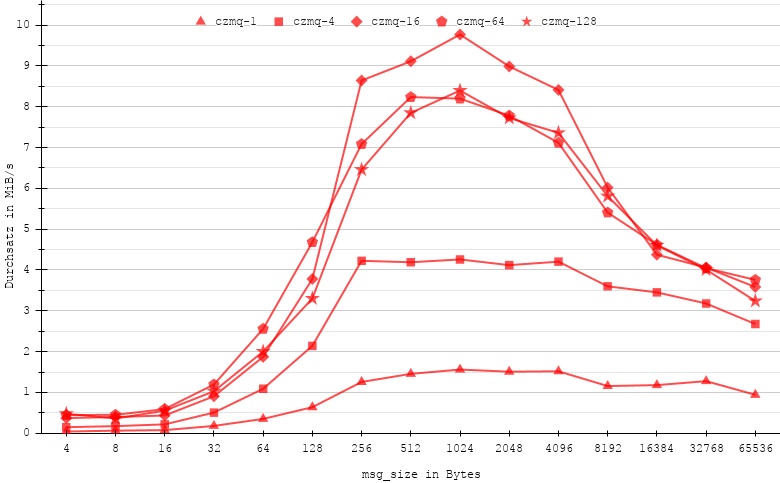
\includegraphics[width=12cm]{images/chart(1).png}
\caption{ZeroMQ Durchsatz abhängig von \texttt{worker\_count} (TCP)}
\end{figure}

\subsection{nanomsg}

Der Durchsatz der nanomsg Implementierung nimmt ebenfalls mit
zunehmender \texttt{msg\_size} zu. Eine steigende Anzahl an Clients sorgt für einen Steigenden Durchsatz, bis zu einer Größe von ca. 64 Clients. Im Gegensatz zu ZeroMQ fällt mit
zusätzlicher Erhöhung von Clients der Durchsatz kaum.

Der höchste gemessene Durchsatz bei nanomsg beträgt 1333 MiB/s mit 64
Clients und einer \texttt{msg\_size} von 64KiB.

\begin{figure}[htbp]
\centering
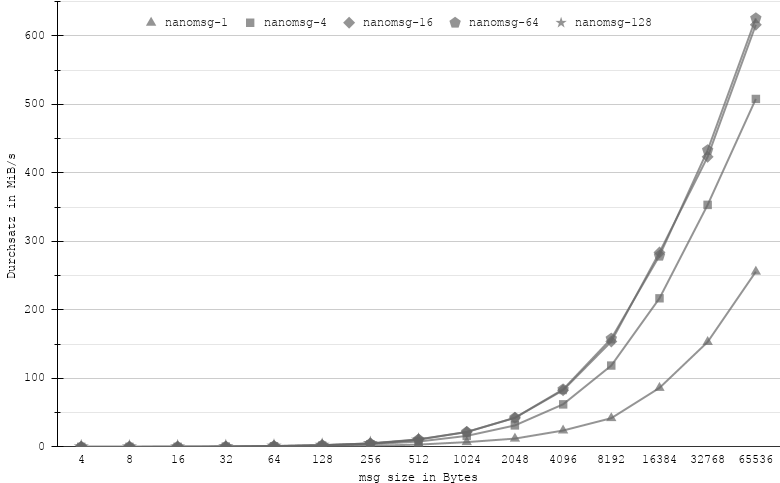
\includegraphics[width=12cm]{images/chart(2).png}
\caption{nanomsg Durchsatz abhängig von \texttt{worker\_count} (TCP)}
\end{figure}

\begin{figure}[htbp]
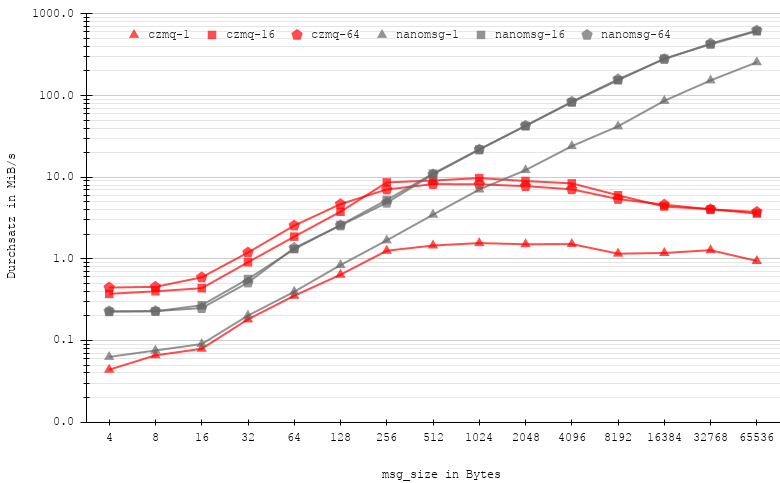
\includegraphics[width=12cm]{images/chart(3).png}
\caption{Durchsatz von ZeroMQ und nanomsg im Vergleich abhängig von \texttt{worker\_count}}
\end{figure}

\subsection{TCP vs IPC}

Mit IPC kann ein Speedup zwischen 0.98 und 1.72 gemessen werden. Der
Durchschnitt aller 107 Messpunkte beträgt ca. 1.28, der Median liegt bei
ca. 1.27. Die Messungen schwanken stark und es lässt sich kein
unmittelbares Muster erkennen.

Besonders groß ist der Speedup bei kleinen Nachrichten und vielen Workern. 
Dies könnte auf den kleineren Overhead von IPC gegenüber TCP zurückzuführen
sein. 

\begin{figure}[htbp]
\centering
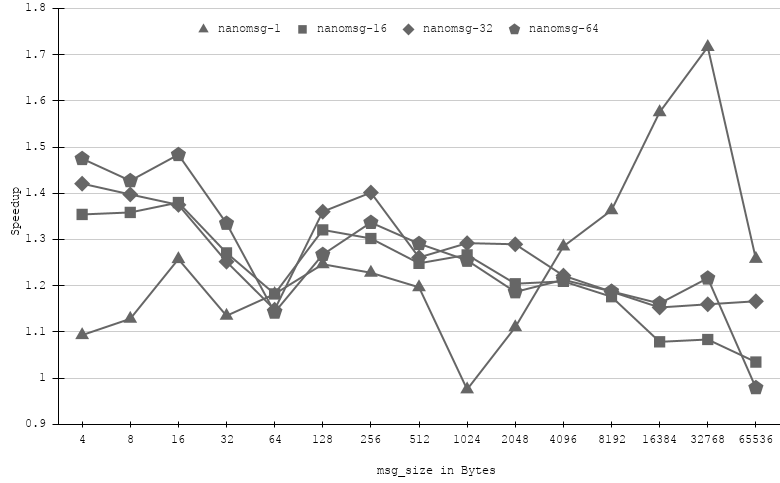
\includegraphics[width=12cm]{images/chart(4).png}
\caption{Speedup IPC gegenüber TCP bei unterschiedlicher \texttt{worker\_size}}
\end{figure}

\section{Diskussion}

Es wurden keine Punkte festgestellt, an dem eine Erhöhung der \texttt{msg\_size} den Durchsatz senkt. Vermutlich wird eine noch höhere \texttt{msg\_size} benötigt. Andere Forscher 
scheinen diese Grenze bei genau 64KiB festgemach zu haben \cite{barroso_benchmarking_2016}. 
Zwischen 4 und 8 Byte ist ein Plateau zu sehen welches durch die verhältnismäßig 
kleine Größe der Nachricht zum Bibliotheks- und Protokoll-Header zu erklären sein könnte.

ZMQ unterliegt nanomsg bei einem Worker um 5-15\%, holt diesen Verlust
bei mehreren Workern allerdings schnell raus. So ist ZeroMQ mit 32 Workern 
in bereits 20-40\% schneller.

Beide Tools erreichen für Grischa ausreichende Durchsätze von über 1333 MiB/s (nanomsg) bzw. 
1444 MiB/s (ZeroMQ). Das Fehlverhalten bei nanomsg ab 128 Workern und 1 KiB
wäre für einen Produktivbetrieb bedenklich, gerade wenn die Nachrichtengröße
dynamisch ist.

Der Speedup von IPC gegenüber TCP ist mit Durchschnittlich 28\% als
moderat aber eindeutig zu bewerten. Gerade bei kleinen Nachrichten kann IPC Punkten. 

Aufgrund des geringen Speedups von IPC kann es Vorteilhaft sein von vornherein 
auf TCP zu setzen, um eine spätere Reimplementierung zu verhindern, sofern
man sich Entscheidet die Anwendungen auf verteilte Systeme zu verlagern. 
Da der Umstieg bei nanomsg von IPC auf TCP (und andersherum) einen 
Geringen Aufwand mitbringt, trifft dies besonders auf ZeroMQ zu.
Grund\-sätz\-lich kann man starke Schwankungen in den Daten erkennen. 

Das Grischa Projekt nutzt im TCP Protokoll meist Nachrichten von 
ca. 64-128 Bytes Länge
mit einer möglichst großen Menge an Workern. In diesem Bereich hat
nanomsg ca. 50\% des Durchsatzes von ZeroMQ. Ein Umstieg auf nanomsg 
aufgrund dieser Metrik allein ist nach diesen Messungen nicht ratsam.
Über die Nachrichten im IPC Protokoll fällt es schwerer ein Urteil zu fällen,
da ZeroMQ nicht mit IPC arbeiten wollte. 

\section{Zusammenfassung}

ZeroMQ und nanomsg bieten einen ähnlichen Durchsatz. 
nanomsg hat die Oberhand bei einem Worker, ZeroMQ mit mehreren. 
Da nanomsg, im Gegensatz zu ZeroMQ, nicht alle Testläufe erfolgreich
abschließen konnte, scheint ZeroMQ das reifere oder auch nur 
einfachere Tool zu sein.

Nur nanomsg konnte mit sowohl TCP als auch IPC getestet werden. Hier
konnte ein Speedup von durchschnittlich 28\% erzielt werden. Die
Ergebnisse unterliegen allerdings großen Schwankungen.

Im Einsatzbereich des Grischa Projekts (kleine Nachrichten, viele
Worker) wird beim Umstieg auf nanomsg der Datendurchsatz sinken. Ein
Umstieg ist aufgrund dieser Metrik nicht Ratsam.

\section{Ausblick}

Die Ergebnisse stützen sich auf eine Request-Reply Pattern mit Broker
während Grischa ein komplexeres Publish-Subscribe Pattern 
mit Broker nutzt (XPubXSub). Eine Implementierung vom XPubXSub
könnte Sicherheit schaffen, dass sich die Performance unter
diesen Umständen ähnlich verhält. 

Die Benchmarks wurden nur auf einer Node ausgeführt. Um 
den Aufbau weiter an Grischa anzulehnen, müssten die Nodes 
Real auf unterschiedlichen Systemen laufen.

nanomsg hat einen Nachfolger namens nng ("nanomsg-next-gen"). Diese Reimplementierung verspricht 
Verlässlichkeit und Skalierbarkeit \cite{noauthor_nanomsgnng_2021}. Eine Ge\-gen\-ü\-ber\-stell\-ung
zu nanomsg könnte interessante Ergebnisse bringen.
\clearpage

\bibliographystyle{plain}
\bibliography{references}

\listoffigures

\end{document}